% TikZ/pgfplots redraws of the diagrams in Test_answers.pdf (Q1 removed, so
% question numbers here are the NEW numbers 1-6).
% ---- Q1 (ASRJC 2025 P1 Q7): circle x^2+y^2=4 and line sqrt3 y = x+2 -------------
% \figTcircle{variant}: 0 = question, 1 = solution (a), 2 = solution (b)
\newcommand{\figTcircle}[1]{%
\begin{tikzpicture}
\begin{axis}[qfig, trig format=deg, width=7.4cm, height=6.6cm, axis equal image, xmin=-3.2, xmax=3.4, ymin=-2.6, ymax=3.1]
  \ifnum#1<2
    \fill[blue!22] plot[domain=60:180, samples=60, variable=\t] ({2*cos(\t)},{2*sin(\t)}) -- cycle;
  \else
    \fill[blue!22] (axis cs:1,{sqrt(3)}) -- (axis cs:2,{4/sqrt(3)}) -- (axis cs:2,0)
       -- plot[domain=0:60, samples=40, variable=\t] ({2*cos(\t)},{2*sin(\t)}) -- cycle;
  \fi
  \addplot[curve, domain=0:360, samples=120, variable=\t] ({2*cos(\t)},{2*sin(\t)});
  \addplot[line2, domain=-3:3.1] {(x+2)/sqrt(3)};
  \node[below left] at (axis cs:0,0) {$O$};
  \node[right] at (axis cs:3.0,2.85) {$\sqrt{3}y=x+2$};
  \node[below right] at (axis cs:0.6,-1.35) {$x^2+y^2=4$};
  \ifnum#1<2 \node[above left, inner sep=1pt] at (axis cs:1.1,1.95) {$\left(1,\sqrt{3}\right)$};\fi
  \ifnum#1=1
    \draw[dashed, thin] (axis cs:1,-2.4) -- (axis cs:1,2.6);
    \node[below left] at (axis cs:-2,0) {$-2$};
    \node[below right] at (axis cs:1,0) {$1$};
  \fi
  \ifnum#1=2
    \draw[thin] (axis cs:2,-2.4) -- (axis cs:2,3);
    \draw[dashed, thin] (axis cs:-2.6,{4/sqrt(3)}) -- (axis cs:2.6,{4/sqrt(3)});
    \draw[dashed, thin] (axis cs:-2.6,{sqrt(3)}) -- (axis cs:2.6,{sqrt(3)});
    \node[left] at (axis cs:0,2.55) {$\frac{4}{\sqrt{3}}$};
    \node[left] at (axis cs:0,1.55) {$\sqrt{3}$};
    \node[below right] at (axis cs:2,0) {$2$};
  \fi
\end{axis}
\end{tikzpicture}}

% ---- Q2 (DHS 2025 P1 Q6) ------------------------------------------------------------
\newcommand{\figTtriangle}{%
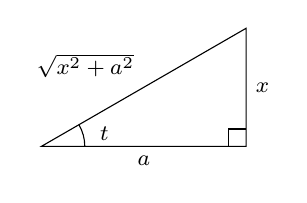
\begin{tikzpicture}[scale=1.0, every node/.style={font=\footnotesize}]
  \draw[thin] (0,0) -- (2.6,0) -- (2.6,1.5) -- cycle;
  \draw[thin] (2.38,0) -- (2.38,0.22) -- (2.6,0.22);
  \draw[thin] (0.55,0) arc[start angle=0, end angle=30, radius=0.55];
  \node at (0.8,0.16) {$t$};
  \node[below] at (1.3,0) {$a$};
  \node[right] at (2.6,0.75) {$x$};
  \node[above left] at (1.3,0.75) {$\sqrt{x^2+a^2}$};
\end{tikzpicture}}
\newcommand{\figTdhs}{%
\begin{tikzpicture}
\begin{axis}[qfig, width=7.2cm, height=6.4cm, xmin=-1.5, xmax=1.6, ymin=-1.75, ymax=1.75]
  \addplot[curve, domain=-0.995:0.995] {x*sqrt(x^2+1)};
  \node[circle, draw, fill=white, inner sep=1.2pt] at (axis cs:1,{sqrt(2)}) {};
  \node[circle, draw, fill=white, inner sep=1.2pt] at (axis cs:-1,{-sqrt(2)}) {};
  \node[above right] at (axis cs:1,{sqrt(2)}) {$\left(a,\sqrt{2}a\right)$};
  \node[below left] at (axis cs:-1,{-sqrt(2)}) {$\left(-a,-\sqrt{2}a\right)$};
  \node[below right] at (axis cs:0,0) {$O$};
  \node at (axis cs:-0.75,0.75) {$y=\dfrac{x\sqrt{x^2+a^2}}{a}$};
\end{axis}
\end{tikzpicture}}

% ---- Q3 (RI 2025 P1 Q10): y = 2 - x/sqrt(2x-1) -----------------------------------
% \figTri{variant}: 0 = question, 1 = (b)(i) labelled + parabola, 2 = (b)(ii) region R, 3 = (c)(iii) region S
\newcommand{\figTri}[1]{%
\begin{tikzpicture}
\begin{axis}[qfig, width=11.5cm, height=6.6cm, xmin=-0.4, xmax=9, ymin=-2.4, ymax=3.3, restrict y to domain=-3:4]
  \ifnum#1=2
    \fill[black!15] plot[domain=1:3, samples=60] ({\x},{2-\x/sqrt(2*\x-1)}) -- (axis cs:3,0.5) -- (axis cs:1,0.5) -- cycle;
  \fi
  \ifnum#1=3
    \fill[black!15] plot[domain=1:4, samples=60] ({\x},{2-\x/sqrt(2*\x-1)}) -- (axis cs:4,0) -- (axis cs:3,0)
       -- plot[domain=3:1, samples=60] ({\x},{1-sqrt((\x-1)/2)}) -- cycle;
  \fi
  \addplot[curve, domain=0.5012:0.62, samples=120] {2-x/sqrt(2*x-1)};
  \addplot[curve, domain=0.62:8.6, samples=200] {2-x/sqrt(2*x-1)};
  \draw[asym] (axis cs:0.5,-2.4) -- (axis cs:0.5,3.2);
  \ifnum#1=1
    \addplot[line2, smooth, domain=-1.1:3.1, samples=80, variable=\t] ({2*(\t-1)^2+1},{\t});
    \node[right] at (axis cs:0.5,3.0) {$x=\frac{1}{2}$};
    \node[pt] at (axis cs:1,1) {};
    \node[above left] at (axis cs:1,1.05) {$(1,1)$};
    \node[below right] at (axis cs:0.536,0) {$(0.536,0)$};
    \node[below] at (axis cs:3,-0.05) {$(3,0)$};
    \node[above] at (axis cs:7.46,0.05) {$(7.46,0)$};
    \node[right] at (axis cs:4.6,2.75) {$x=2(y-1)^2+1$};
    \node at (axis cs:2.3,-1.8) {$y=2-\frac{x}{\sqrt{2x-1}}$};
  \else\ifnum#1=0
    \node at (axis cs:3.0,1.75) {$y=2-\frac{x}{\sqrt{2x-1}}$};
  \fi\fi
  \ifnum#1=2
    \addplot[line2, domain=0:8.6] {0.5};
    \draw[thin] (axis cs:1,-2.4) -- (axis cs:1,3.2);
    \draw[thin] (axis cs:3,-2.4) -- (axis cs:3,3.2);
    \node[left] at (axis cs:0,0.5) {$0.5$};
    \node[below right] at (axis cs:1,0) {$1$};
    \node[below right] at (axis cs:3,0) {$3$};
  \fi
  \ifnum#1=3
    \addplot[line2, smooth, domain=-1.1:3.1, samples=80, variable=\t] ({2*(\t-1)^2+1},{\t});
    \draw[thin] (axis cs:1,-2.4) -- (axis cs:1,3.2);
    \draw[thin] (axis cs:4,-2.4) -- (axis cs:4,3.2);
    \node[below left] at (axis cs:1,0) {$1$};
    \node[below] at (axis cs:3,0) {$3$};
    \node[below right] at (axis cs:4,0) {$4$};
    \node[right] at (axis cs:5.6,0.45) {$y=2-\frac{x}{\sqrt{2x-1}}$};
    \node[right] at (axis cs:5.6,-1.75) {$y=1-\sqrt{\frac{x-1}{2}}$};
  \fi
  \node[below left] at (axis cs:0,0) {$O$};
\end{axis}
\end{tikzpicture}}

% ---- Q4 (TMJC 2025 P1 Q8): y = 5-(x-3)^2, normal y = -x/2+5 --------------------------
\newcommand{\figTtmjc}{%
\begin{tikzpicture}
\begin{axis}[qfig, width=7.4cm, height=9cm, xmin=-1.2, xmax=6.5, ymin=-5.6, ymax=6.4]
  \fill[red!30] (axis cs:0,5) -- (axis cs:2,4) -- (axis cs:0,4) -- cycle;
  \fill[blue!22] (axis cs:0,4) -- plot[domain=2:0, samples=60] ({\x},{5-(\x-3)^2}) -- cycle;
  \addplot[curve, domain=-0.2:6.2, samples=150] {5-(x-3)^2};
  \addplot[line2, domain=-1:6.3] {-x/2+5};
  \node[pt] at (axis cs:0,5) {};
  \node[pt] at (axis cs:3,5) {};
  \node[pt] at (axis cs:2,4) {};
  \node[pt] at (axis cs:0,-4) {};
  \node[left] at (axis cs:0,5.15) {$(0,5)$};
  \node[above] at (axis cs:3,5) {$(3,5)$};
  \node[below right] at (axis cs:2,3.9) {$(2,4)$};
  \node[left] at (axis cs:0,-4) {$(0,-4)$};
  \node[below left] at (axis cs:0,0) {$O$};
  \node[right] at (axis cs:3.6,2.9) {$y=-\frac{1}{2}x+5$};
  \node[right] at (axis cs:1.35,-2.5) {$x=-\sqrt{5-y}+3$};
\end{axis}
\end{tikzpicture}}

% ---- Q5 (VJC 2025 P1 Q9): x = 6-(y-2)^2, y = 2-x, y = 8 ---------------------------
\newcommand{\figTvjc}{%
\begin{tikzpicture}
\begin{axis}[qfig, width=10cm, height=8.2cm, xmin=-7.6, xmax=8.2, ymin=-2.6, ymax=10]
  \fill[blue!22] plot[domain=0:5, samples=60] ({6-(\x-2)^2},{\x}) -- cycle;
  \addplot[curve, smooth, domain=-2.2:6.3, samples=100, variable=\t] ({6-(\t-2)^2},{\t});
  \addplot[line2, domain=-7.3:4.6] {2-x};
  \addplot[black, thin, domain=-7.3:7.5] {8};
  \node[pt] at (axis cs:6,2) {};
  \node[right] at (axis cs:6,2) {$(6,2)$};
  \node[below left] at (axis cs:0,0) {$O$};
  \node at (axis cs:-1.4,6.6) {$R$};
  \node at (axis cs:2.4,2.2) {$S$};
  \node[above] at (axis cs:4.5,8) {$y=8$};
  \node[right] at (axis cs:-5.8,9.4) {$y=2-x$};
  \node[below] at (axis cs:-4.5,-1.2) {$x=6-(y-2)^2$};
\end{axis}
\end{tikzpicture}}

% ---- Q6 (EJC 2025 P1 Q5): y = 1/x, rectangles on [1,2] -----------------------------
% \figTejc{0 = under the curve (question), 1 = above the curve (solution (d))}
% x' = 6(x-1)+1.6 cm, y' = 2.3y cm; broken x-axis between the y-axis and x = 1
\newcommand{\figTejc}[1]{%
\begin{tikzpicture}[every node/.style={font=\footnotesize}]
  \foreach \a/\b in {1/1.1, 1.1/1.2, 1.8/1.9, 1.9/2} {
    \ifnum#1=0 \pgfmathsetmacro\h{2.3/\b}\else\pgfmathsetmacro\h{2.3/\a}\fi
    \pgfmathsetmacro\xa{6*(\a-1)+1.6}\pgfmathsetmacro\xb{6*(\b-1)+1.6}
    \draw[rect] (\xa,0) rectangle (\xb,\h);}
  \draw[blue, semithick, smooth, domain=0.75:2.45, samples=80] plot ({6*(\x-1)+1.6},{2.3/\x});
  \draw[black!45, thin] (0,0) -- (0.55,0) -- (0.65,-0.12) -- (0.75,0.12) -- (0.85,0) -- (8.2,0);
  \draw[ax3] (8.1,0) -- (8.3,0) node[right, black!60] {$x$};
  \draw[ax3] (0,0) -- (0,3.3) node[above, black!60] {$y$};
  \draw[dashed, thin] (1.6,0) -- (1.6,3.1);
  \draw[dashed, thin] (7.6,0) -- (7.6,3.1);
  \node[below] at (1.6,0) {$1$};
  \node[below] at (7.6,0) {$2$};
  \node at (4.6,0.25) {$\cdots$};
  \node[below] at (4.6,0) {$\cdots$};
  \node[right] at (7.9,1.3) {$y=\frac{1}{x}$};
\end{tikzpicture}}

% =====================================================================
% Task 8 (2026 swap-ins). Numbers below are the NEW test numbers.
% ---- Q1 (ACJC 2026 P1 Q6): y = f(x) on [0,1], f(x) = e^{-2x}/(1+e^{-2x}) -------------
% \figTlim{variant}: 0 = question (region A shaded), 1 = solution (b) (n lower rectangles)
\newcommand{\figTlim}[1]{%
\begin{tikzpicture}
\begin{axis}[qfig, width=7.4cm, height=5cm, xmin=-0.05, xmax=1.22, ymin=0, ymax=0.62, xtick=\empty, ytick=\empty]
  \addplot[region, domain=0:1, samples=40] {exp(-2*x)/(1+exp(-2*x))} \closedcycle;
  \ifnum#1=1
    \foreach \k in {1,2,3,6,7,8} {\edef\tmp{\noexpand\draw[rect] (axis cs:{(\k-1)/8},0) rectangle (axis cs:{\k/8},{exp(-2*\k/8)/(1+exp(-2*\k/8))});}\tmp}
    \node[below] at (axis cs:0.125,0) {$\frac{1}{n}$}; \node[below] at (axis cs:0.25,0) {$\frac{2}{n}$};
    \node[below] at (axis cs:0.5,-0.01) {$\cdots$}; \node at (axis cs:0.5,0.08) {$\cdots$};
    \node[below] at (axis cs:0.75,0) {$\frac{n-2}{n}$}; \node[below] at (axis cs:0.875,0) {$\frac{n-1}{n}$};
  \fi
  \addplot[curve, domain=0:1, samples=40] {exp(-2*x)/(1+exp(-2*x))};
  \draw[thin] (axis cs:1,0) -- (axis cs:1,{exp(-2)/(1+exp(-2))});
  \node[below left] at (axis cs:0,0) {$0$}; \node[below] at (axis cs:1,0) {$1$};
  \node[above right] at (axis cs:0.78,0.2) {$y=\mathrm{f}(x)$};
  \ifnum#1=0 \node at (axis cs:0.45,0.18) {$A$};\fi
\end{axis}
\end{tikzpicture}}

% ---- Q2 (TMJC 2019 P2 Q4, modified): x = -sqrt(t^2+4), y = ln t / t -----------------------
\newcommand{\figTparam}{%
\begin{tikzpicture}
\begin{axis}[qfig, width=8cm, height=5.4cm, xmin=-5.4, xmax=0.6, ymin=-1.1, ymax=0.55, xtick=\empty, ytick=\empty]
  \addplot[region, domain=1:3, samples=50, variable=\t] ({-sqrt(\t*\t+4)},{ln(\t)/\t}) -- (axis cs:{-sqrt(13)},0) -- (axis cs:{-sqrt(5)},0) -- cycle;
  \addplot[curve, domain=0.45:12, samples=120, variable=\t] ({-sqrt(\t*\t+4)},{ln(\t)/\t});
  \draw[thin, dashed] (axis cs:{-sqrt(13)},-0.9) -- (axis cs:{-sqrt(13)},0.5);
  \draw[thin, dashed] (axis cs:{-sqrt(5)},-0.9) -- (axis cs:{-sqrt(5)},0.5);
  \fill (axis cs:{-sqrt(e*e+4)},{1/e}) circle (1.3pt);
  \node[above] at (axis cs:{-sqrt(e*e+4)},{1/e}) {$\left(-\sqrt{\mathrm{e}^2+4},\frac{1}{\mathrm{e}}\right)$};
  \node[below right] at (axis cs:{-sqrt(5)},0) {$-\sqrt{5}$}; \node[below left] at (axis cs:{-sqrt(13)},0) {$-\sqrt{13}$};
  \node[below left] at (axis cs:0,0) {$O$}; \node[right] at (axis cs:-1.95,-0.75) {$C$};
\end{axis}
\end{tikzpicture}}

% ---- Q4 (ACJC 2026 P2 Q5): y = sin^{-1}(1-x), 0<=x<=2, drawn as x = 1 - sin y ------------
% \figTasin{variant}: 1 = (b)(i) areas A and R, 2 = (b)(ii) region R and the cylinder
\newcommand{\figTasin}[1]{%
\begin{tikzpicture}
\begin{axis}[qfig, width=6.8cm, height=6cm, xmin=-0.5, xmax=2.6, ymin=-1.9, ymax=1.9, xtick=\empty, ytick=\empty]
  \ifnum#1=1 \addplot[region, domain=0:pi/2, samples=40, variable=\t] ({1-sin(\t)},{\t}) -- (axis cs:0,0) -- cycle;\fi
  \addplot[region, domain=-pi/2:0, samples=40, variable=\t] ({1-sin(\t)},{\t}) -- (axis cs:2,0) -- cycle;
  \addplot[curve, domain=-pi/2:pi/2, samples=60, variable=\t] ({1-sin(\t)},{\t});
  \draw[thin, dashed] (axis cs:0,{-pi/2}) -- (axis cs:2,{-pi/2});
  \node[left] at (axis cs:0,{pi/2}) {$\frac{\pi}{2}$}; \node[left] at (axis cs:0,{-pi/2}) {$-\frac{\pi}{2}$};
  \node[above] at (axis cs:1,0) {$1$}; \node[above right] at (axis cs:2,0) {$2$};
  \node[below left] at (axis cs:0,0) {$O$};
  \ifnum#1=1 \node at (axis cs:0.28,0.45) {$A$};\fi
  \node at (axis cs:1.72,-0.45) {$R$};
\end{axis}
\end{tikzpicture}}

% ---- Q6 (RI 2026 P1 Q9): y = x e^{-x} --------------------------------------------------------
% \figTxex{variant}: 1 = (b) sketch, 2 = (c) R and S, 3 = (d) translated down 2 units
\newcommand{\figTxex}[1]{%
\ifnum#1=3 \def\sh{-2}\def\ylo{-2.4}\def\yhi{0.3}\def\fh{7.5cm}\else\def\sh{0}\def\ylo{-0.05}\def\yhi{0.55}\def\fh{5cm}\fi
\begin{tikzpicture}
\begin{axis}[qfig, width=7.2cm, height=\fh, xmin=-0.3, xmax=5.2, ymin=\ylo, ymax=\yhi, xtick=\empty, ytick=\empty]
  \ifnum#1=2
    \addplot[region, domain=0:1, samples=40] {x*exp(-x)} -- (axis cs:1,{1/e}) -- (axis cs:0,{1/e}) -- cycle;
    \draw[thin, dashed] (axis cs:1,0) -- (axis cs:1,{1/e}); \node at (axis cs:0.65,0.12) {$S$}; \node at (axis cs:0.18,0.31) {$R$};
  \fi
  \ifnum#1=3
    \addplot[region, domain=0:1, samples=40] {x*exp(-x)-2} -- (axis cs:1,{1/e-2}) -- (axis cs:0,{1/e-2}) -- cycle;
    \draw[thin, dashed] (axis cs:0,-2) -- (axis cs:5,-2); \node[below] at (axis cs:4.2,-2) {$y=-2$};
    \node at (axis cs:0.2,-1.75) {$R'$};
  \fi
  \ifnum#1>1 \draw[thin] (axis cs:0,{1/e+\sh}) -- (axis cs:2.2,{1/e+\sh}); \fi
  \addplot[curve, domain=0:5, samples=60] {x*exp(-x)+\sh};
  \fill (axis cs:1,{1/e+\sh}) circle (1.3pt);
  \ifnum#1=3 \node[above] at (axis cs:1.3,{1/e-2}) {$\left(1,\frac{1}{\mathrm{e}}-2\right)$}; \node[above] at (axis cs:3.4,-1.8) {$y=x\mathrm{e}^{-x}-2$};
  \else \node[above right] at (axis cs:1,{1/e}) {$\left(1,\frac{1}{\mathrm{e}}\right)$}; \node[right] at (axis cs:2.4,0.24) {$y=x\mathrm{e}^{-x}$};\fi
  \ifnum#1=2 \node[right] at (axis cs:2.2,{1/e}) {$y=\frac{1}{\mathrm{e}}$};\fi
  \node[below left] at (axis cs:0,0) {$O$};
\end{axis}
\end{tikzpicture}}
